
\documentclass[sigconf]{acmart}
%\documentclass{article}
%\usepackage{booktabs} % For formal tables
%\documentclass{article}
%\usepackage{floatrow}
\usepackage{graphicx}
\usepackage{multirow,subfig}
%\usepackage[dvipsnames]{xcolor}
\usepackage{amsfonts}
\usepackage{amsmath}
\usepackage{amssymb}
\usepackage{mathtools}
\usepackage{amssymb}
\usepackage{listings}
%\usepackage{amsthm}
%\usepackage[section]{placeins}
\usepackage{enumitem}
%\usepackage[a4paper, total={7in, 10.5in}]{geometry}
\usepackage{caption}
\usepackage[linesnumbered,ruled]{algorithm2e}
\usepackage{algpseudocode}
\captionsetup{labelfont=bf,textfont=bf}
\usepackage{subfig} % Needs subfig for this example.
%\usepackage[demo]{graphicx}
%\setlength{\footskip}{15pt}
%\usepackage[utf8]{inputenc}
%\usepackage[english]{babel}
\newtheorem{theorem}{Theorem}[section]
\newtheorem{corollary}{Corollary}[theorem]
%\newtheorem{lemma}[theorem]{Lemma}
\newcommand\todo[1]{\textcolor{red}{#1}}
\newcommand\greg[1]{\textcolor{blue}{greg: #1}}

\newcommand*\diff{\mathop{}\!\mathrm{d}}
\newcommand*\Diff[1]{\mathop{}\!\mathrm{d^#1}}

\lstset{language=C,
	keepspaces=true,
	frame=tb,
	basicstyle=\ttfamily,
	columns=fixed,
	morekeywords={enddo},
	mathescape}

\DeclareSymbolFont{matha}{OML}{txmi}{m}{it}% txfonts
\DeclareMathSymbol{\varS}{\mathord}{matha}{83}


% Copyright
%\setcopyright{none}
%\setcopyright{acmcopyright}
%\setcopyright{acmlicensed}
%\setcopyright{rightsretained}
%\setcopyright{usgov}
%\setcopyright{usgovmixed}
%\setcopyright{cagov}
%\setcopyright{cagovmixed}


% DOI
\acmDOI{}

% ISBN
\acmISBN{}

%Conference
\acmConference[SPAA'18]{ACM SPAA conference}{February 2018}{Vienna, Aurstria} 
\acmYear{2018}
\copyrightyear{2018}

\newcommand\myeq{\stackrel{\mathclap{\normalfont\mbox{def}}}{=}}
\newcommand\myineq{\stackrel{\mathclap{\normalfont\mbox{?}}}{\leq}}
\newcommand{\specialcell}[2][c]{%
	\begin{tabular}[#1]{@{}c@{}}#2\end{tabular}}

\newtheorem{mydef}{Definition}

%\title{Automatic creation of I/O lower bound for statically analyzable 
%programs}
%\author{Grzegorz Kwasniewski}
\begin{document}
	\title{Yet another Matrix Multiplication paper}
		
	\author{Grzegorz Kwasniewski}
	\affiliation{%
		\institution{ETH Zurich}
%		\streetaddress{P.O. Box 1212}
%		\city{Dublin} 
%		\state{Ohio} 
%		\postcode{43017-6221}
	}
	\email{gkwasnie@inf.ethz.ch}
	
			\author{Marko Kabic}
	\affiliation{%
		\institution{CSCS}
		%		\streetaddress{P.O. Box 1212}
		%		\city{Dublin} 
		%		\state{Ohio} 
		%		\postcode{43017-6221}
	}
	\email{marko.kabic@cscs.ch}
	
			\author{Joost VandeVondele}
	\affiliation{%
		\institution{CSCS}
		%		\streetaddress{P.O. Box 1212}
		%		\city{Dublin} 
		%		\state{Ohio} 
		%		\postcode{43017-6221}
	}
	\email{joost.vandevondele@cscs.ch}
	
		\author{Torsten Hoefler}
	\affiliation{%
		\institution{ETH Zurich}
		%		\streetaddress{P.O. Box 1212}
		%		\city{Dublin} 
		%		\state{Ohio} 
		%		\postcode{43017-6221}
	}
	\email{htor@inf.ethz.ch}
	
	\begin{abstract}
In this paper we address an allegedly well-known problem of distributed Matrix 
Matrix Multiplication and show new optimizations both from theoretical and 
implementation sides. We establish a new framework for 
assessing 
analytical data movement lower bounds, together with deriving optimal 
sequential and parallel scheduling. Our "bottom-up" parallelization technique, 
opposed to state of the art "top-down" approaches is naturally agnostic to 
problem dimensions and is provably optimal in all scenarios, resulting in up to 
$\sqrt{3}$ times reduction in communication volume. With our 
fine-tuned data layout 
transformations, we are able to achieve X \% peak FLOP/s running on up to Y 
nodes on the Piz Daint supercomputer, beating currently fastest-known 
algorithms by a factor of Z. \greg{Computation and communication overlap. will 
add this once we have it.}
%Based on an existing pebble game 
%abstraction, we come 
%to fundamental observations about parallel scheduling and data reuse, deriving 
%new tiling scheme for Matrix-Matrix Multiplication, achieving a tight bound of 
%$\frac{2mnk}{\sqrt{S}}$ I/O operations. We show the new NP-hardness 
%proof for I/O optimal scheduling.
	\end{abstract}

\keywords{I/O complexity, scheduling, pebble games}


\maketitle

%	\maketitle
	
%	\tableofcontents
	
	\section{Introduction}
	Matrix multiplication kernel is one of the most fundamental building blocks 
	in linear algebra and even slightest optimizations have vast impact. The 
	evolution of matrix multiplication algorithms goes through tiling, 
	parallelization, Strassen-like routines, and non-square matrices. We note 
	that even though most recent works, like CARMA (cite), achieve asymptotic 
	lower bounds for all configurations of dimensions and intra-node memory 
	sizes, the recursive structure of the algorithm is not suitable for 
	scenarios when the number of processes is not the power of two. 
	Furthermore, we emphasize that in practical considerations, asymptotic 
	complexity is insufficient, as constants may play crucial role in 
	applicability of algorithms (confront, e.g., Coppersmith–Winograd algorithm 
	(cite) ). We are able to outperform the current state-of-the art 
	implementations in all scenarios by a factor of up to $\sqrt{3}$ in terms 
	of communication volume and up to X in the total runtime. The 
	implementation 
	also addresses the challenges of recursive data layout of CARMA which 
	prohibits transparent integration with ScaLAPACK format and yields 
	suboptimal computation throughput.
	
	Even though the final schedule generated by our framework resembles CARMA, 
	we took entirely different approach that is provably I/O optimal and easily 
	generalizable to other linear algebra kernels (\greg{should we include 
	others, like LU or Cholesky?}).
 \greg{Computation and communication overlap. will add this once we have it.}
	
%	It is a well known fact that the main emphasis on performance analysis 
%	shifted from maximizing FLOP/s to minimizing data movement. Even though I/O 
%	optimal schemes were being designed since the first register problems 
%	occurred (\cite{pebblegameregister}, \cite{registerpebblecolor}, 
%	\cite{completeRegisterProblems}, \cite{redblue}, \cite{externalMem}), 
%	contemporary throughput-oriented architectures, like Xeon Phi 
%	\cite{XeonPhi} and GPUs 
%	\cite{gpumodel} leveraged the problem to higher importance than ever 
%	(\cite{redbluewhite}, \cite{elangoSymbolic}, \cite{energyScheduling}, 
%	\cite{communicationOptMMM}). Yet, 
%	data movement minimization, due to its 
%	combinatorial nature, is far more complicated than simple FLOP/s 
%	optimization.
%	
%	As a starting point we revisit a method proposed by Hong and Kung nearly 40 
%	years 
%	ago \cite{redblue}. Their red-blue pebble game abstraction is 
%	a simple, yet elegant and powerful tool for analyzing the I/O complexity of 
%	computations expressed in the Computation Directed Acyclic Graph (CDAG) 
%	format. The key result is a method of  deriving the I/O lower bound based 
%	on a so-called \textit{S-partition} of the input CDAG.
%	
%	In this work we show the new NP-hardness result of the
%	S-partition problem. We also discuss the origin of the problem 
%	intractability and summarize cases where either polynomial time or PTAS 
%	algorithm exists. For those cases, the polynomial time algorithm is 
%	presented. However, we note that for many practical scenarios, the constant 
%	$k$ in the exponent of time complexity $\mathcal{O}(n^k)$ may still be 
%	prohibitive. To tackle 
%	this obstacle, we derive a new ILP-based branch-and-bound algorithm 
%	inspired by a 
%	work of Elango et al. (\cite{redbluewhite}) that can scale to graphs with 
%	up to (to be evaluated) vertices. 
%	
%	There are two major challenges with the S-partition. First one is present 
%	in 
%	all methods that maximizes computational intensity (the geometric 
%	interpretation is surface-to-volume ratio minimization). The problem is 
%	that those methods do not explicitly specify the data reuse. This leads to 
%	suboptimal subset shapes, which we prove on the Matrix Matrix 
%	Multiplication example.  The other challenge with S-partition lower 
%	bound is that it does not 
%	provide any tightness guarantees. We present a method 
%	to assess both the tightness and scheduling feasibility derived 
%	directly from the S-partition.  We compare our algorithm with both 
%	well-known 
%	results for Matrix-Matrix Multiplication, FFT and stencil computations, as 
%	well as random uniform and Kronecker graphs.
%	
%	This paper is organized as follows:
%	
%	(TBD)
%	
%	
	\section{Background}
	\subsection{I/O complexity- pebble games and S-partition}
	\label{sec:background}
	\greg{Drastically reduce this section. What are the parts that should stay?}
	
	This model bases on the work of the red-blue pebble game by Hong and Kong 
	(\cite{redblue}), which was later extended to red-blue-white pebble game by 
	Elango (\cite{redbluewhite}). In this model, computation of a given DAG is 
	represented as graph 
	pebbling with red and blue pebbles. The number of the red pebbles is 
	bounded and represents the size of a fast memory, whereas the blue pebbles 
	represent a slow memory and their number is unlimited. For the exact 
	description of the pebble game, we refer a reader to the original paper. 
	The key feature of this model is that computation is not modeled - the only 
	cost comes from the data movement between the fast and the slow memory. 
	
	DEFINITION 1: (Red-Blue pebble game \cite{redblue}).
	Given a DAG $C = (I,V,E,O)$
	such that any vertex with no incoming (resp.
	outgoing) edge is an element of the input set I (resp. output set O), S red 
	pebbles and
	an arbitrary number of blue pebbles, with a blue pebble on
	each input vertex. A complete game is any sequence of steps
	using the following rules that results in a final state with blue
	pebbles on all output vertices:
	\begin{itemize}
		\item R1 (Input)
		A red pebble may be placed on any vertex that has
		a blue pebble (load from slow to fast memory),
		\item R2 (Output)
		A blue pebble may be placed on any vertex that
		has a red pebble (store from fast to slow memory),
		\item R3 (Compute)
		If all immediate predecessors of a vertex of
		$V - I$ have red pebbles, a red pebble may be placed on that
		vertex (executing operation),
		\item R4 (Delete)
		A red pebble may be removed from any vertex
		(reuse storage).
	\end{itemize}
	
	
	The extension presented by Elango is twofold: it introduces one relaxation 
	and one restriction. It relaxes the original problem by introducing a 
	flexible input/output vertex labeling - not all the input (and output) 
	vertices must have a blue pebble at the beginning (and end) of computation.
	The restriction prohibits recomputation of the nodes by introducing the 
	white pebbles. Once a red pebble has been placed on a node using the 
	computation rule, it can only be stored (by placing a blue pebble) or 
	loaded (by placing a red pebble on a blue pebble). Therefore, there is a 
	change in rule \textbf{R3 (Compute)} : \textit{If a vertex v does not have 
		a white pebble and
		all its immediate predecessors have red pebbles on them, a
		red pebble along with a white pebble may be placed on v.}
	
%	\subsubsection{Pebble game and I/O complexity}
	Each valid pebble game corresponds to the valid schedule of I/O operations. 
	As many of the scheduling problems, the general case is NP hard 
	\cite{RedBlueHard}. 
	Furthermore, to the best of our knowledge, there is no closed form 
	optimization function that represents the optimal pebble game.
	
	Hong and Kung introduced the concept of \textit{S-Partitioning}, which 
	divides the whole computation DAG into consecutive subcomputations which 
	requires at least fixed amount of I/O operations. Red-blue-white pebble 
	extension allows to reason more strictly about the subsets' boundaries 
	(we refer the reader to the original papers).
	
	Let $I \subseteq V$ be the set of vertices with fan-in 0 and $O \subseteq 
	V$ be the set 
	of vertices with fan-out 0. Then:
	
	DEFINITION 2:  (S-partition of a CDAG \cite{redbluewhite}).
	Let $G = (I,V,E,O)$ be a computation DAG (CDAG). An S-partition of $G$ 
	is a 
	collection of 
	$h$ subsets of $V - I$ such that:
	
	\begin{itemize}
		\item P1: $\cap_{i=1}^{h} V_i=\emptyset$ and $\cup_{i=1}^{h} V_i=V$
		\item P2: there is no cyclic dependence between subsets.
		\item P3: $\forall i, |In(V_i)| \le S$
		\item P4: $\forall i, |Out(V_i)| \le S$
	\end{itemize}
	where $In(V_i) = \{u \in V - V_i : \exists_{v \in V_i}(u,v) \in E \}$ and 
	$Out(V_i) = \{u \in V_i: \exists{v \in V - V_i} (u,v) \in E \}$
	
	Now if the number of red pebbles (the size of the fast memory) is S, we can 
	see that each subset in the 2S-Partition requires at 
	least S I/O operations to execute (2S comes from a fact that maximum 
	possible reuse between the subsets is at most S, so at least additional S 
	pebbles have to be loaded). By finding the minimum number of 
	those subsets, we can derive the I/O lower bound:
	
	LEMMA 1: (Lower bound on I/O \cite{redblue}). Let $H(2S)$ be the minimal 
	number of 
	vertex sets for any valid 2S-partition of a given CDAG. Then the minimal 
	number Q of I/O operations for any valid execution of the CDAG is bounded 
	by	
	\begin{equation}
	\label{eq:redbluebound}
	Q \ge S \times (H(2S) - 1)
	\end{equation}
	We refer a reader to the original paper for a complete proof, but here we 
	sketch the idea: for each subcalculation $C_1$ of the input DAG that 
	requires exactly $S$ transitions using rule R1 or R2, we define two subsets 
	of $V$, $V_{R,i}$ and $V_{BR,i}$ as 
	follows:
	\begin{enumerate}
		\item $V_{R,i}$ consists of those vertices that have red pebbles placed 
		on 
		them just before subcalculation $C_i$ begins.
		\item $V_{BR,i}$ consists of those vertices that have blue pebbles 
		placed 
		on them just before subcalculation $C_i$ begins and have red pebbles 
		placed on them according to rule R1 during $C_i$.
	\end{enumerate}
	
	Then, we can derive the following observations:
	\begin{enumerate}
		\item $V_{R,i} \cup V_{BR,i} = Dom(V_i)$
		\item $|V_{R,i}| \le S$
		\item $|V_{BR,i}| \le S$
		\item $|V_{R,i} \cup V_{BR,i}| \le |V_{R,i}| + |V_{BR,i}| \le 2S$
	\end{enumerate}
	
	An example subset of a 3-point stencil 8-partition is shown in Figure 
	\ref{fig:spart-stencil}.
	
	\begin{figure}
		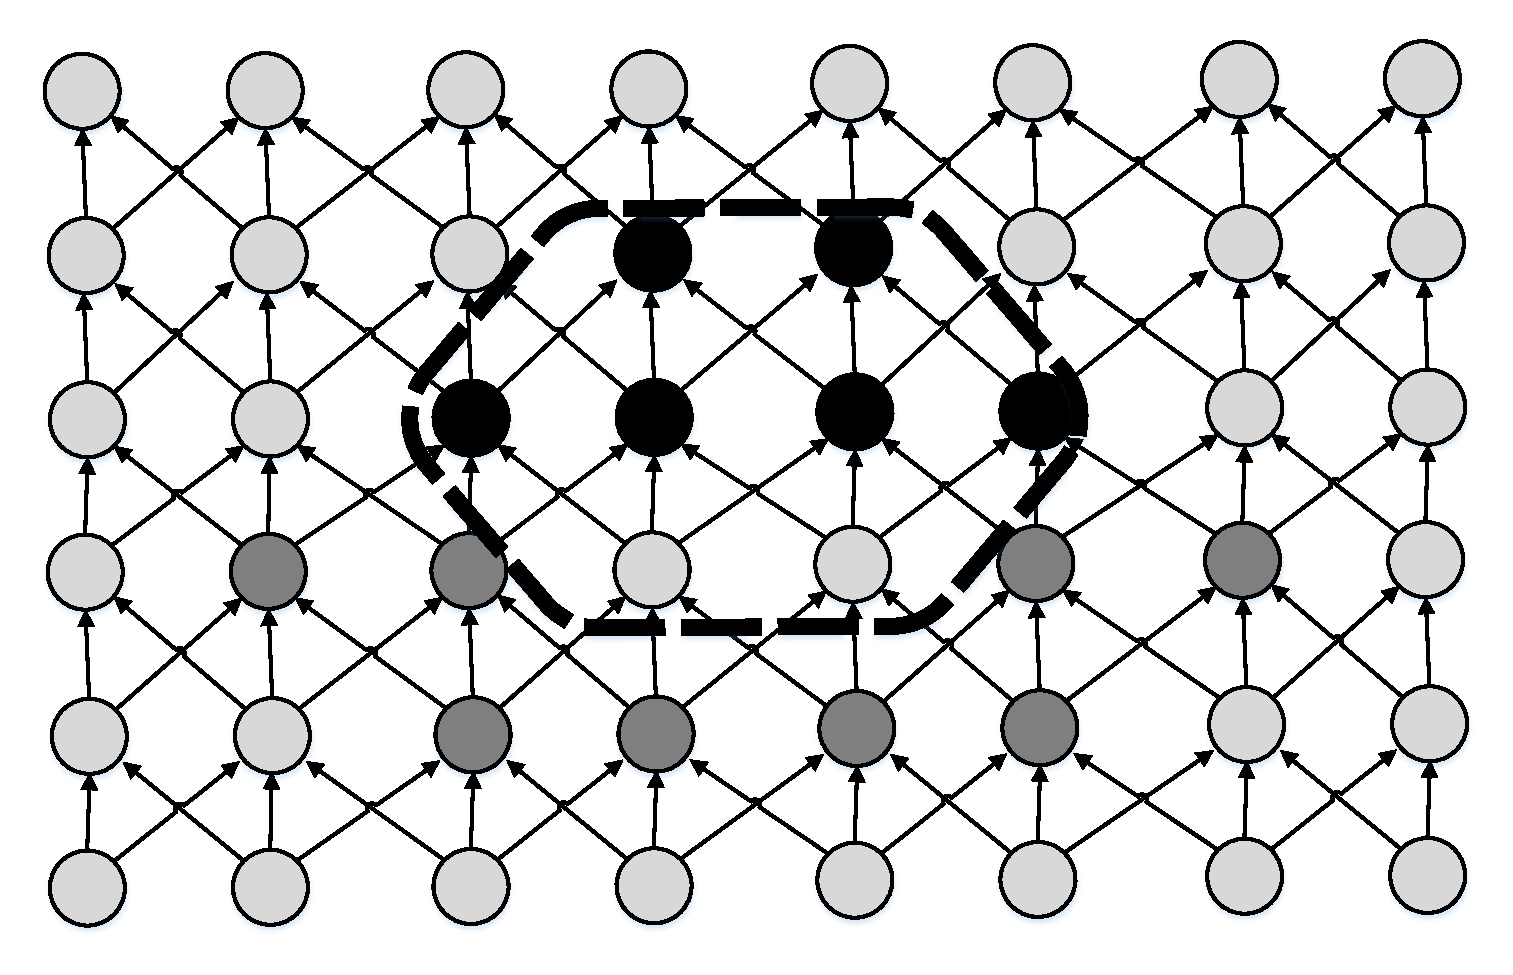
\includegraphics[width=2\columnwidth/3]{figures/stencils}
		\caption{A valid subset of a 3-point stencil 8-partition (outlined with 
		black dashed line), with $|In| = 8$ (dark gray vertices) and $|Out| = 
		6$ (black vertices). Lemma 1 states that having $8/2 = 4$ red pebbles, 
		at least 4 I/O operations are required to execute this subset.}
		\label{fig:spart-stencil}
	\end{figure}

\subsection{Matrix multiplication?}
\greg{I'm not sure if we need background on this. Maybe linear algebra in 
general?}	

\section{NP-hardness proof of the S-partition problem}
\label{sec:np-hard}

\greg{I think we don't need this at all here}

In this section we show the polynomial time reduction of the well-known bin 
packing problem, which is strongly NP-hard
(\cite{computersIntractability}), to the S-partition problem.

\begin{mydef}
	Bin packing problem (\cite{computersIntractability}). 
	
	INSTANCE. Finite set $U$ of items, a size $s(i) \in Z$ for each $i \in U$, 
	a positive integer bin capacity $B$, and a positive integer $K$.
	
	QUESTION. Is there a partition of $U$ into disjoint sets $U_1, U_2, ..., 
	U_k$ such that the sum of sizes of the items in each $U_i$ is $B$ or less?
\end{mydef}

Because the bin packing problem is strongly NP-hard, we restrict the vertex 
sizes to be encoded in the unary notation.

We construct the corresponding S-partition instance as following (Figure 
\ref{fig:spartition_binpacking}):
\begin{enumerate}
	\item For each $1 \le i \le n$ create a gadget as following:
	\begin{itemize}
		\item Add $B+1$ input and middle vertices $u_{i, j}$ and $v_{i, j}$ for 
		$j = 1..B+1$ 
		and add directed edge between each pair of vertices from different 
		group: $\forall_{j,k = 
		1..B+1}u_{i,j},v_{i,k} \in E$.
		\item Add $s(i)$ output vertices $w_{i, s(i)}$ and connect every vertex 
		$v_{i,k}$ to all $w_{i,m}$ : $\forall_{j = 
			1..B+1, k = 1..s(i)}v_{i,j},w_{i,k} \in E$.
	\end{itemize}
	\item Create an instance $\mathcal{I}$ of S-partition problem on the 
	resulting graph 
	with $S = B$.
\end{enumerate}

The corresponding graph has $2(B+1)n + s(a)+s(b)+...+s(n)$ vertices and 
$(B+1)^2 n + \sum_{i = 1..n}(B+1)s(i)$ edges and hence its size is polynomial 
in the size 
of the corresponding bin packing problem.

\textit{Claim:}
In decision problem $\mathcal{I}$, each of the gadgets is contained in a single 
S-partition subset. 
The problem asks can we merge those gadgets into $K$ S-partitions so that $S = 
B$.

\textit{Proof: }
We show that by the definition of S-partition, each of the gadgets has to 
be contained in one subset with the empty input set. Let's assume 
opposite that there is a valid S-partition in which there is a gadget contained 
in more than one subset. Consider such gadget $i$ corresponding to item $i$ of 
size $s(i)$.
Without loss of generality assume that $0 \le a \le B+1$ input vertices 
$u_{i}$, $0 \le b \le B+1$ middle vertices $v_{i}$ and $0 \le c \le s(i)$ 
output 
vertices $w_{i}$, $0 < a + b + c < 2B + 1 + s(i)$ belong to subset $p1$ and the 
remaining vertices of the gadget belong to $p2$. Now we have two cases: if $a 
\cdot b = 
0$, then partition $p1$ would have $B+1$ inputs or outputs, because a whole 
layer containing $B+1$ would have to be connected. If $a \cdot b > 0$, then 
there would be a cyclic dependence between partitions $p1$ and $p2$, a 
contradiction. \qed

The solution of the problem $\mathcal{I}$ can be directly translated to the 
corresponding solution of Bin packing problem : $\forall_{i = 1..n} b(i) = 
p(g(i))$, where $b(i)$ is a bin number in which item $i$ is placed, $g(i)$ is a 
gadget $i$ in Problem $\mathcal{I}$ and $p(g(i))$ is a subset number in which 
gadget $i$ is contained.

\begin{figure}
	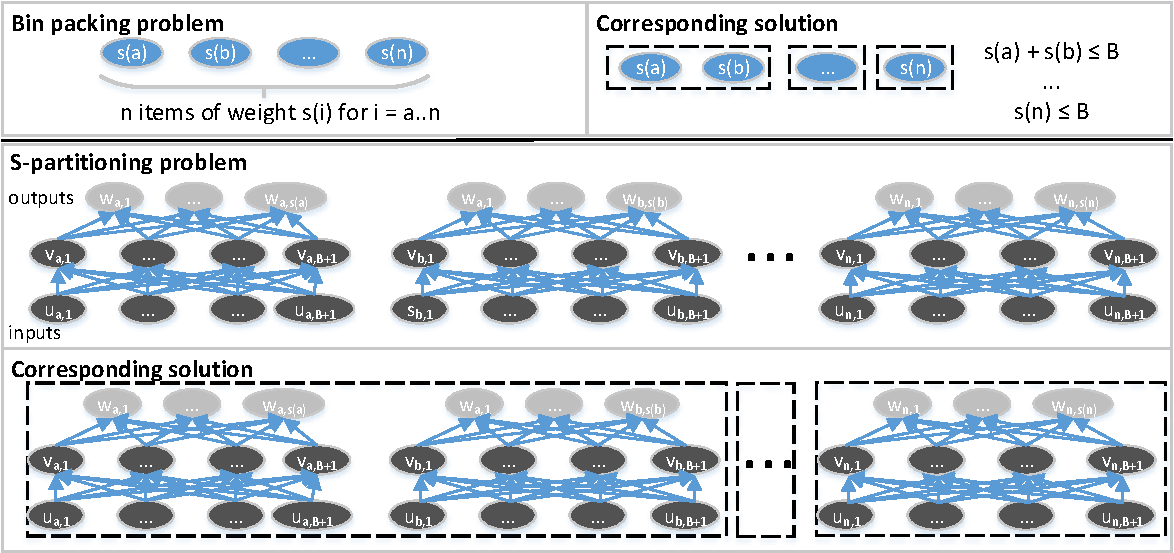
\includegraphics[width=\columnwidth]{figures/spartitioning_nphard3}
	\caption{The Reduction of the bin packing problem to the S-partition 
	problem.}
	\label{fig:spartition_binpacking}
\end{figure}


\textbf{Discussion:} \todo{make it more formal}

\begin{enumerate}
	\item Although bin packing is NP-hard to approximate within a factor of 3/2 
	- $\epsilon$, there exists an asymptotic PTAS algorithm solving the problem 
	(that is, when the number of bins is sufficiently large) 
	\cite{binpackingPTAS}. It is worth noting, however, that the running time 
	of this algorithm is infeasible for most real problems.
	\item Yue (\cite{binpackingApprox}) proved that the first fit decreasing 
	heuristics running in $O(n \log 
	n)$ time use no more than 11/9 \textbf{OPT} + 1 bins.
	\item If bin size is fixed (therefore, for fixed S), there exists a 
	pseudo-polynomial time algorithm 
	of complexity $k^{p(0)+p(1)+\dots+p(B)}$, which checks all possible ways to 
	assign a number of bins to each of possible ways how to partition numbers 
	$0 \dots B$ into an unordered sum of positive integers ( $p(i)$ is the 
	partition function and represents the number of possible partitions of 
	natural number $i$).
	\item Encoding item weights with corresponding number of vertices requires 
	unary weight representation. Still, Jansen et al. 
	(\cite{unaryBinPacking}) showed that unary bin packing problem is W[1]-hard.
	\item All those observations suggests that there is a greedy 
	heuristic for S-partition which is guaranteed to be at most constant 
	multiplicative factor off the optimal solution. We will present such 
	algorithm and its correctness proof in Section \ref{sec:approx-algo}.
\end{enumerate}

	\section{2S-Partition, S-Partition and data reuse}
\label{sec:Svs2S}

\greg{I think this can be also skipped}

The reasoning behind 2S-Partition accounts for an upper bound of data 
reuse 
between subsets.
This, however, can lead to underestimation. With a slight modification of 
the original proof, we show that finding the minimum number of subsets in 
S-Partition 
(instead of 
2S-Partition) gives the correct, and tighter, lower bounds, but it 
requires better model of data reuse, and therefore, finding optimal order 
of execution of the subsets.

LEMMA 2:
the minimal number Q of I/O operations for any valid execution of the CDAG 
is bounded by	
\begin{equation}
Q \ge (S - R(S)) \times (H(S) - 1)
	\label{eq:reusebound}
\end{equation}

where $R(S)$ is an upper bound on the reuse volume between the subsets.

\textit{Proof:}

It suffices to observe that, by the definition $R(S)$, we have:
$$\forall_{i} V_{R} \le R(S)$$
and rewrite the observation (4) as $|V_{R,i}| - |R(S)| \le S$ \qed


%	
%	The "safe" approach using 2S instead of S, forces each partition to perform 
%	at least S load operations due to the size of the dominator set (at most S 
%	vertices from the dominator set could be loaded at the start of the $i$th 
%	computation). 
%	However, to compute each partition optimally (the only I/O operations are 
%	at the inputs and output nodes of the partition), we often need all S red 
%	pebbles to be used by the subcalculation $C_i$. This is the case for the 
%	partitions, where at least one of the output vertices $v$ depend on all the 
%	input vertices [ref]. Then, if the number of inputs is $S$, there are at 
%	least $S$ disjoint paths from the inputs to $v$, which require at least $S$ 
%	active red pebbles to pebble $v$. Therefore, after each subcalculation 
%	$C_i$, all the red pebbles must be moved from $V_i$ to $V_{i+1}$, requiring 
%	$S$ I/O operations.
%	
\subsection{Data reuse and a subset shape}
\label{sec:partitionShape}

\greg{Although this is an old work from the spartition paper, it's easy to show 
that CARMA asymptotically reaches \textbf{cubic} scheme, which can be up to 
$\sqrt{3}$ times slower than \textbf{par. in ijk dim}. Therefore, I would 
rewrite 
this section, but not remove it.}.

The key difference between the original lower bound lemma (inequality 
\ref{eq:redbluebound}) and the lemma presented in this paper (inequality 
\ref{eq:reusebound}) is the explicit notion of reuse. 
If S-partition is to be used for scheduling, instead of just deriving 
(not tight) I/O lower bounds, a problem of fundamental nature occurs.
S-partition approach, as many other methods (e.g., \cite{IronyMMM}, 
\cite{MMM_LW}, \cite{elangoSymbolic}), focuses on maximizing computational 
intensity, 
i.e., number of operations per loaded byte. In geometric interpretation, 
this is a surface to volume minimization, as in Loomis-Whitney inequality 
(\cite{loomisWhitney}). However, surprisingly this may not yield optimal 
results if we 
consider data reuse.

EXAMPLE (Matrix-Matrix Multiplication): For MMM, it is easy to prove that 
the optimal subset shape maximizing computational intensity is a cube 
(Figure \ref{fig:mmmreuse}). If we allow surface to be bounded by S, 
then 
with a simple calculation	
\begin{multline}
\label{eq:cubic}
\\
\mathcal{S}_1 = S \\
3 n_1^2 = S \\
n_1 = \sqrt{\frac{S}{3}} \\
\mathcal{V}_1 = n_1^3 = \Big(\frac{S}{3}\Big)^{\frac{3}{2}} \\
\rho_1 = \frac{\mathcal{V}_1}{\mathcal{S}_1} = \frac{n_1}{3} = 
\sqrt{\frac{S}{18}}\\
\end{multline}

where $\mathcal{S}_1$ is the cubic subset's surface (the dominator set 
size), 
$\mathcal{V}_1$ is the cubic subset's volume (the number of vertices in 
the 
subset) and $\rho_1$ is its computational intensity.

However, after the execution of this subset, only one of the faces of 
this cube can be reused - if the innermost loop is $k$ then we reuse the 
last intermediate result of $C$, if the innermost loop is $i$ then we reuse 
the subset of matrix $B$, otherwise we reuse the subset of matrix $A$ 
(Figure \ref{fig:mmm_reuse}). Therefore, maximum possible reuse size $r_1$ 
is 
$n_1^2$, yielding 

$$\rho_{r,1} = \frac{\mathcal{V}_1}{\mathcal{S}_1 - r} = \frac{n_1}{2} = 
\sqrt{\frac{S}{12}}$$

Where $\rho_{r,1}$ stands for the cubic subset computational intensity 
when maximum 
possible reuse is considered. Now consider a "flat" subset, when we load 
a subset of only one column of $A$, one row of $B$ and we compute only one 
"level" (one outer product) of $C$. Then, if the innermost loop is $i$ or 
$j$, we will reuse a single row or single column, giving the reuse size of 
$n_2$, but if the innermost loop is $k$, the reuse is $n_2^2$. Then we 
have: 	
\begin{multline}
\label{eq:flat}
\\
\mathcal{S}_2 = S \\
2n_2 + n_2^2 = S \\
n_2 = \sqrt{S + 1} - 1 \approx \sqrt{S} \\
\mathcal{V}_2 = n_2^2 = (\sqrt{S + 1} - 1)^2  \approx S\\
\rho_2 = \frac{\mathcal{V}_2}{\mathcal{S}_2} = \frac{(\sqrt{S + 1} - 
	1)^2}{2\sqrt{S+1} - 2 + (\sqrt{S + 1} - 1)^2} \approx 1\\
r_2 = n_2^2 \\
\rho_{r,2} = \frac{\mathcal{V}_2}{\mathcal{S}_2 - r_2} = \frac{(\sqrt{S + 
		1} - 
	1)^2}{2\sqrt{S+1} - 2} \approx \sqrt{\frac{S}{4}} 
\end{multline}	
Which gives $\sqrt{3}$ improvement over the cubic shape. We can obtain same 
result if we consider the reuse among other two axes and choose the 
projection of the computation volume to this axis to be $n_2^2$, and other 
projections to be $n_2$. However, in those cases additional 
$\frac{mnk}{\sqrt{S}}$ 
store operations are required for intermediate results of the matrix $C$, 
creating Read-After-Write (RAW) conflicts. This 
observation shows that subset shape 
optimization must be performed together with explicit scheduling and reuse 
formulation to generate an optimal solution.

Following this observation, we can directly derive tight I/O bounds for 
Matrix-Matrix multiplication. Observe that $\rho_r = 
\frac{\mathcal{V}}{\mathcal{S}}$ is a maximum computational intensity for a 
given scheme. Substituting $\mathcal{V}$ by the whole computation domain $n^3$ 
(or $mnk$ for rectangular matrices), we immediately obtain $\mathcal{S}_1 = 
\frac{2\sqrt{3}mnk}{\sqrt{S}}$ for cubic subsets and $\mathcal{S}_1 = 
\frac{2mnk}{\sqrt{S}}$ for flat subsets. Note that this gives a tight 
leading term in a well known asymptotic bound (\cite{redblue}) 
$\Omega\big(\frac{mnk}{\sqrt{S}}\big)$.

\begin{figure}
	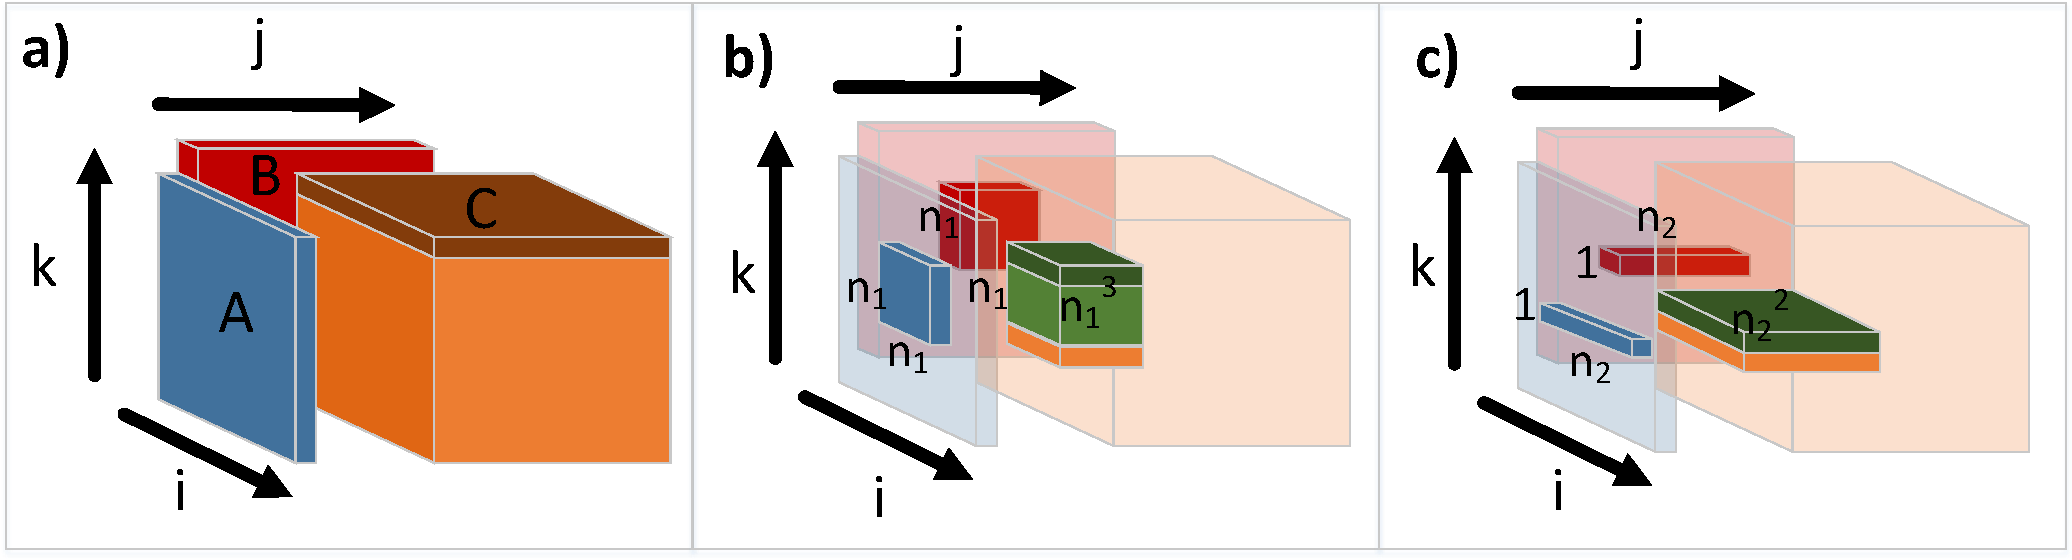
\includegraphics[width=\columnwidth]{figures/mmm_reuse}
	\caption{Matrix-matrix multiplication subset shape problem. a) 
		geometric interpretation of $C = A \times B$ (orange cube represents 
		3-dimensional iteration space of partial sums, matrix C is formed by 
		reduction over dimension $k$ - represented by dark orange plane). b) 
		optimal surface to volume subset shape. Note that in a subsequent 
		subset computation only one of the three planes (blue, red or dark 
		green) can be reused. c) one of three optimal subset shapes when 
		data reuse is considered.}
	\label{fig:mmmreuse}
\end{figure}

The explicit notion of reuse effects not only sequential execution, as 
discussed above, but also parallel scheduling. The number of dependency-free 
subsets in the optimal S-partition determines maximum degree of parallelism up 
to which optimal computational efficiency is maintained. Above this threshold, 
further parallelization is performed either by parallelizing dependent subsets, 
causing additional communication between processes, or by shrinking the size of 
subsets.
 Due to size constraints, the thorough analysis of different parallelization 
 schemes is presented in the Appendix.  Here we show only a comparison of 
 execution time (assuming that each I/O operation takes unit time and every 
 other operation is performed instantaneously) and parallel efficiency of three 
 schemes: 
\begin{enumerate}
	\item \textbf{par. in ij dim:} Subset size is determined by Equation 
	\ref{eq:flat}. 
	The reduction among the \textbf{k} 
	dimension is performed by a single process. Above the maximum degree of 
	parallelism threshold the 
	subsets' size is reduced.
	\item \textbf{par. in ijk dim:} The subset's size is constant determined by 
	Equation \ref{eq:flat}, above the 
	threshold the reduction among the \textbf{k} dimension is parallelized.
	\item \textbf{cubic:} The subset's size is constant determined by Equation 
	\ref{eq:cubic}, above the threshold 
	the reduction among the \textbf{k} dimension is parallelized.
\end{enumerate}

\begin{table}[t]
	\label{tab:mmmEfficiency}
	\caption{Running time and parallel efficiency of the Matrix-Matrix 
		multiplication for different partition schemes. Three ranges correspond 
		to thresholds above which parallelization in \textbf{k} dimension is 
		performed.}
	\begin{tabular}{l|l|l|l|l}
		range & metric & par in \textbf{ij} dim &par. 
		in \textbf{ijk} dim & cubic \\
		%		& $t(p,S)$ & $E(p,S)$ & $t(p,S)$ & $E(p,S)$ & $t(p,S)$ & 
		%$E(p,S)$ \\
		\hline
		\multirow{2}{*}{$p \le \frac{nm}{S}$} & $t(p,S)$ & 
		$\frac{2nmk}{p\sqrt{S}}$ & $\frac{2nmk}{p\sqrt{S}}$ & 
		$\frac{2\sqrt{3}nmk}{p\sqrt{S}}$ \\
		& $E(p,S)$ & 1 & 1 & 	$\frac{1}{\sqrt{3}}$\\
		\hline
		\multirow{2}{*}{$\frac{nm}{S} < p \le \frac{3nm}{S}$} & $t(p,S)$ & $2k 
		\sqrt{\frac{nm}{p}}$ & 
		$\frac{2nmk}{p\sqrt{S}} + S$ &  $\frac{2\sqrt{3}nmk}{p\sqrt{S}}$  
		\\		
		& $E(p,S)$ & $\sqrt{\frac{nm}{pS}}$ & $\frac{1}{1 + 
			\frac{pS^{3/2}}{2nmk}}$ & 	$\frac{1}{\sqrt{3}}$ \\
		\hline
		\multirow{2}{*}{$\frac{3nm}{S} < p$} & $t(p,S)$ & $2k 
		\sqrt{\frac{nm}{p}}$ & 
		$\frac{2nmk}{p\sqrt{S}} + S$ & $\frac{2\sqrt{3}nmk}{p\sqrt{S}} + 
		\frac{S}{3}$\\
		& $E(p,S)$ &	$\sqrt{\frac{nm}{pS}}$ & $\frac{1}{1 + 
			\frac{pS^{3/2}}{2nmk}}$ &	$\frac{1}{\sqrt{3} + 
			\frac{pS^{3/2}}{6nmk}}$
	\end{tabular}
\end{table}


\begin{figure*}[t]
	\hspace*{-1.5cm}
	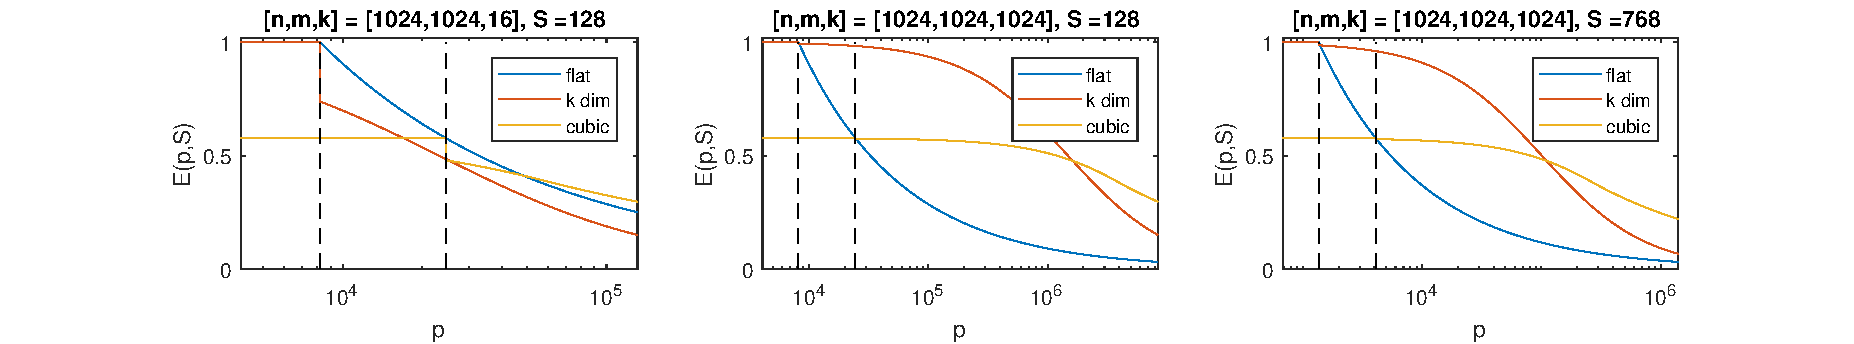
\includegraphics[width=2.5\columnwidth]{figures/mmmScaling}
	\label{fig:mmmScaling}
	\caption{Parallel efficiency of different partition schemes for matrix 
		matrix multiplication. Two vertical dashed lines correspond to 
		thresholds 
		$nm/p$ and $3nm/p$ (Table \ref{tab:mmmEfficiency}).}
\end{figure*}

\section{CARMA 2.0 ?}
 \greg{Computation and communication overlap. will add this once we have it.}
\subsection{Recursive vs single step}
\begin{enumerate}
	\item \greg{Recursive steps determine data layout.}
	\item \greg{Manual reduction tree vs MPI collectives. Conclusion: We 
	implemented both, but on Piz daint recursive is faster, possibly due to 
	static knowledge about spatial data locality}
\end{enumerate}
\subsection{Local buffer reuse}
\greg{We use two buffers instead of $\log P$}
\subsection{Block recursive data layout}
\begin{enumerate}
	\item \greg{Faster, doesn't require reshuffling in each step}
	\item \greg{Better suitable for integration with ScaLAPACK ?}
\end{enumerate}


\section{Evaluation}
\subsection{Test cases}
\greg{Describe where do the skinny matrices show up, why they are important, 
why strong scaling (even suboptimal) is important.}
\subsection{Environment}
\greg{Piz daint description}
\subsection{Results}
\greg{I believe the scenarios should cover, both weak and strong scaling (I 
don't know in which order):
\begin{itemize}
	\item "Standard" square scenario. Marko - we are still the fastest even for 
	square case?
	\item "CARMA" scenarios. Power of 2, one and two "large dimensions"
	\item "Our case" scenarios. Non power of 2, rectangular matrices. Is it 
	fair to assume that original CARMA pads matrices with zeros to match the 
	closest power of 2?
\end{itemize}
Should we add intra node evaluation too? Or do we care only about the 
distributed case?
}

\section{Related work}
\begin{enumerate}
	\item \greg{I/O minimization in general, starting from pebble games, to 
	communication minimization in linear algebra.}
	\item \greg{Asymptotic complexity and the importance of constants.}
	\item \greg{Matrix multiplication algorithms.}
\end{enumerate}


%	To the best of our knowledge, in the literature there is a disparity 
%	between the work-centric and communication-centric scheduling. The former 
%	one focuses on minimizing the execution critical path by reordering and 
%	splitting tasks among the processing units (\cite{schedulingNP}). Many 
%	related scheduling problems are formulated as knapsack  
%	\cite{knapsackSched}, 
%	\cite{knapsackQuadSched} or partially ordered 
%	knapsack \cite{POKSched} optimization. Communication-centric (or 
%	communication-avoiding) approach tries to minimize the number and volume of 
%	messages exchanged across processes (e.g, \cite{SchedMaxFlow}). Many 
%	problem-specific methods are 
%	known, e.g. in linear algebra \cite{mmmSched}, \cite{communicationOptMMM}, 
%	\cite{Cholesky}, PDE solvers \cite{MeshPart} or 
%	stencil computations \cite{modesto}. For 
%	general DAG scheduling, however, the focus is mostly on different variants 
%	of balanced min-cuts of graphs \cite{balancedGraphPart}, 
%	\cite{dagPartitioningTrees}. This approach 
%	indeed lowers the 
%	communication overhead while trying to distribute work evenly. Even though 
%	balanced graph partition is also known to be NP-hard 
%	\cite{schedHardness}, \cite{partitioningHardness}, much work 
%	has been done to improve the efficiency of approximation algorithms 
%	\cite{approximatingCuts}, \cite{balancedGraphPart}.
%	
%	I/O minimizing scheduling focuses on maximizing data reuse - both spatial 
%	and temporal. Spatial data reuse orbits around vectorization and alignment 
%	techniques. Temporal reuse requires instruction reordering, like loop 
%	tiling or loop fusion. Those techniques are widely used in stencil 
%	computations (\cite{modesto}) and linear algebra 
%	(\cite{comm-avoiding-triang}). Abstractions like polyhedral model 
%	(\cite{polyhedralModel}) 
%	give powerful 
%	mathematical tools to e.g., minimize reuse distance, but they are 
%	limited to only particular class of programs. Elango et. al 
%	(\cite{redbluewhite}) worked on general class represented by CDAG, but the 
%	authors 
%	focused on I/O lower bound, without assessing its tightness or generating 
%	schedules.
%	In this work, we try to combine those two approaches. In the work-centric 
%	view, a computation DAG is viewed in a context of dependencies between the 
%	tasks and a goal is to minimize the depth - therefore, partitions tend to 
%	be aligned with a critical path. In the communication centric view, a cut 
%	size is minimized, which can result in partitions perpendicular to a 
%	critical path - loosing the grasp on the overall execution time.

\section{Conclusions}

%\section{Notes}
%NP-hardness, approximation algorithms. Is S-partition submodular ? If so, 
%look at "Fast Greedy Algorithms in MapReduce and Streaming".
%

%	\section{Bibliography}
\bibliographystyle{IEEEtran}
\bibliography{mmm}

\appendix
\section{Parallel scheduling}
\todo{Move the whole thing to appendix? Or discard it?}
In this section, we start with the reuse analysis from Section 
\ref{sec:partitionShape} 
to derive the execution time and parallel efficiency metric of the two tiling 
schemes of Matrix-Matrix multiplication. In this framework, we assume that each 
I/O operation takes unit time and any arithmetic operation is performed 
instantaneously, therefore $t = Q$. We start with two observations:

\begin{enumerate}
	\item There is only one dimension on 
	which a reuse set projection is not empty $\exists!_{\mathbf{d}}: 
	\phi_{\mathbf{d}}(R) \ne 
	\emptyset$, which implies, that there is no reuse along the plane 
	perpendicular 
	to this dimension. Furthermore, if $\mathbf{d} = \mathbf{k}$, meaning that 
	$\mathbf{m} \times \mathbf{n} \parallel \mathbf{k}$, then if the 
	parallelization is performed only on the \textbf{mn} plane, then there are 
	no RAW 
	conflicts discussed in Section \ref{sec:partitionShape} - subsets on 
	this 
	plane are embarrassingly parallel. 
	\item To achieve maximum reuse (and therefore optimum usage 
	of the fast memory), the subset shape must be fixed to the one derived 
	in 
	Section \ref{sec:partitionShape}. This means, that there is maximum 
	available 
	parallelism (dictated by the number of optimal subsets in one  
	\textbf{mn} plane) up to which the parallel efficiency will remain 
	constant. Above this threshold, we have three options: 1) reduce the 
	subset size, reducing the effective memory size, 2) parallelize in 
	\textbf{k} dimension, creating RAW writes and requiring additional 
	communication between processes, 3) create cubic subsets, effectively 
	combining 1 and 2.
\end{enumerate}

From this, we derive following formulas:

\begin{multline}
\\
a_0 = \sqrt{S+1} - 1   \text{ (size of a side of the square subset )}\\
N = \frac{nm}{a^2} \approx \frac{nm}{S}  \text{ (number of optimal square 
	subsets in one \textbf{mn} plane)}\\
D_0(p,S) = |\{P \in \mathcal{P} : \forall_{P_i, P_j} \phi_{\mathbf{k}}(P_i) = 
\phi_{\mathbf{k}}(P_j)\}| = k \\
\text{number of subsets which projection along the \textbf{k} dimension is 
	equal} \\ 
\text{- because the subsets are flat, the "height" of the 
	subset stack}
\\ 
\text{in \textbf{k} dimension is k }\\
\end{multline}

Now, for the case where we do not exceed the parallelism threshold  $p \le N$ : 
\begin{multline}
\\
t_0(p,S) = \frac{N}{p} (\mathcal{S}_0 - r_0) D_0(p,S) = \frac{2nmk(\sqrt{S+1} 
	- 
	1)}{(\sqrt{S+1} - 1)^2 p} \approx \frac{2nmk}{\sqrt{S} p}  \\
E_0(p,S) = \frac{t_0(1,S)}{p t_0(p,S)} = 1 \\
\end{multline}

If  $p > N$, we have two previously discussed cases: smaller square tiles and 
parallelization in \textbf{k} dimension. Case 1:
\begin{multline}
\\
D_1(p,S) = D_0(p,S) \\
a_1 = \sqrt{\frac{nm}{p}} \text{ size of a side of the reduced square 
	subset} \\
\mathcal{S}_1 - r_1 = 2a_1 = 2\sqrt{\frac{nm}{p}} \text{ number of load 
	operations per one subset} \\
t_1(p,S) = (\mathcal{S}_1 - r_1) D_1(p,S) = 2k \sqrt{\frac{nm}{p}}  \\
E_1(p,S) = \frac{t_0(1,S)}{p t_1(p,S)} = \sqrt{\frac{nm}{Sp}} \\
\end{multline}

Case 2 (parallelization in \textbf{k} dimension): 

\begin{multline}
\\
D_2(p,S) = \frac{D_0(p,S)N}{p} \text{ (the depth is reduced by } \frac{N}{p} 
\text{)}\\
a_2 = a , \mathcal{S}_2 = \mathcal{S}_0\\ 
r_2 = a_2^2(1 - \frac{p}{Nk}) \text{ (in every $\frac{p}{N}$ plane in dimension 
	\textbf{k} we} \\
\text{communicate whole $a_2^2$ plane between subsets)} \\
t_2(p,S) = (\mathcal{S}_2 - r_2) D_2(p,S)  = \frac{2nmk}{\sqrt{S}p} + S  \\
E_2(p,S) = \frac{t_0(1,S)}{p t_2(p,S)} = \frac{1}{1 + \frac{\sqrt{S}p}{2nmk}} \\
\end{multline}

Case 3 (cubic subsets - Section \ref{sec:subsetShape}):

\begin{multline}
\\
a_3 = \sqrt{\frac{S}{3}} \\ 
\mathcal{S}_3 = 3a_3^2, r_3 = a_3^2\\ 
D_3(p,S) = \frac{nmk}{p \Big(\frac{S}{3}\Big)^{\frac{3}{2}}}\\
\\
\frac{nm}{S} \le p < \frac{3nm}{S} :\\
t_3(p,S) = (\mathcal{S}_3 - r_3) D_3(p,S)  = \frac{2\sqrt{3}mnk}{\sqrt{S}p}  \\
E_3(p,S) = \frac{t_1(1,S)}{p t_3(p,S)} =  \frac{1}{\sqrt{3}}\\
\\
p > \frac{3nm}{S} :\\
t_3(p,S) = (\mathcal{S}_3 - r_3) D_3(p,S)  = \frac{2\sqrt{3}mnk}{\sqrt{S}p}  \\
E_3(p,S) = \frac{t_1(1,S)}{p t_3(p,S)} =  \\
\end{multline}

$$2 \cdot h_{Sopt}(G) \ge \sum_{P \in \mathcal{P}(G)} h_{Sopt}(inv(P)) $$
$$ \nexists_{P \in \mathcal{P}}: V_{w,opt} \in P $$

%\begin{algorithm}
%	\label{alg:spartition}
%	\SetKwInOut{Input}{Input}
%	\SetKwInOut{Output}{Output}
%	\underline{rSpartitionCut}\;


\end{document}

